\def\xcoords{{2.0, 4.5, 3.5, 7.0, 5.2, 3.5, 1.7, 4.0, 7.0}}
\def\ycoords{{7.2, 6.9, 8.6, 9.0, 5.6, 4.7, 2.9, 1.8, 3.8}}


\def\labelpos{{225, 80, 90, 45, 285, 200, 225, 270, 315}}
\def\scale{0.5}
\def\offset{0}

\begin{center}
    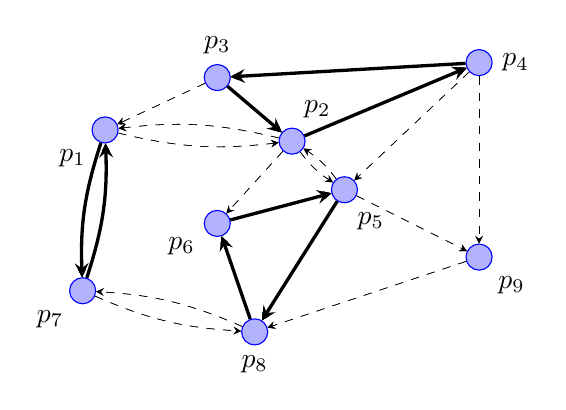
\begin{tikzpicture}[scale=0.95]
    \tikzstyle{vertex} = [circle, draw=blue, fill=blue!30];
    \tikzstyle{arc} = [very thin, draw, dashed, -stealth];
    \tikzstyle{arcbend} = [arc, bend right = 10];
    \tikzstyle{usedarc} = [arc, very thick, solid];
    \tikzstyle{usedarcbend}=[usedarc, bend right=10];   
        
    % Draw instance
    \foreach \i/\j in {1/225, 2/80, 3/90, 4/0, 5/285, 6/200, 7/225, 8/270, 9/315}
    {
        \node[vertex, label=\j:{$p_{\i}$}] (v\i) at (\xcoords[\i-1],\scale * \ycoords[\i-1]) {};
    }
        
    % Draw arcs
    \foreach \i/\j in {2/4, 2/6, 3/1, 3/2, 4/3, 4/5, 4/9, 5/8, 5/9, 6/5, 8/6, 9/8}
    {
        \draw (v\i) edge [arc] (v\j);
    }
    
    % Draw bending arcs
    \foreach \i/\j in {1/2, 1/7, 2/1, 2/5, 5/2, 7/1, 7/8, 8/7}
    {
        \draw (v\i) edge [arcbend] (v\j);
    }
    
    % Draw used straight arcs
    \foreach \i/\j in {2/4, 4/3, 3/2, 5/8, 8/6, 6/5}
    {
        \draw (v\i) edge [arc] (v\j);
    }    
    
    % Draw used bending arcs
    \foreach \i/\j in {1/7, 7/1}
    {
        \draw (v\i) edge [arcbend] (v\j);
    }

    % DRAW A KIDNEY EXCHANGE SOLUTION
    \onslide<+->
    {
        % Draw arcs
        \foreach \i/\j in {2/4, 2/6, 3/1, 3/2, 4/3, 4/5, 4/9, 5/8, 5/9, 6/5, 8/6, 9/8}
            \draw (v\i) edge [arc] (v\j);
        
        % Draw bending arcs
        \foreach \i/\j in {1/2, 1/7, 2/1, 2/5, 5/2, 7/1, 7/8, 8/7}
            \draw (v\i) edge [arcbend] (v\j);
        
        % Draw used straight arcs
        \foreach \i/\j in {2/4, 4/3, 3/2, 5/8, 8/6, 6/5}
            \draw (v\i) edge [usedarc] (v\j);
        
        % Draw used bending arcs
        \foreach \i/\j in {1/7, 7/1}
            \draw (v\i) edge [usedarcbend] (v\j);
    }
    
    
    % \onslide<2>{
    %     %%%%%%%%%%%%%%
    %     %SECOND STAGE%
    %     %%%%%%%%%%%%%%
        
    %     % SATAN!!!
    %     \node[style=devil, minimum size=1cm] (satan) at ($(v5)-(6,0)$) {};
        
    %     % Draw pairs
    %     \node[coveredpair, label=225:$p_{1}$] (v1) at (\xcoords[0], \scale*\ycoords[0]) {};
    %     \node[coveredpair, label=80:$p_{2}$] (v2) at (\xcoords[1], \scale*\ycoords[1]) {};
    %     \node[coveredpair, label=above:$p_{3}$] (v3) at (\xcoords[2], \scale*\ycoords[2]) {};
    %     \node[coveredpair, label=45:$p_{4}$] (v4) at (\xcoords[3], \scale*\ycoords[3]) {};     
    %     \node[coveredpair, label=285:$p_{5}$] (v5) at (\xcoords[4], \scale*\ycoords[4]) {};
    %     \node[coveredpair, label=200:$p_{6}$] (v6) at (\xcoords[5], \scale*\ycoords[5]) {};
    %     \node[coveredpair, label=225:$p_{7}$] (v7) at (\xcoords[6], \scale*\ycoords[6]) {};
    %     \node[coveredpair, label=below:$p_{8}$] (v8) at (\xcoords[7], \scale*\ycoords[7]) {};
    %     \node[pair, label=315:$p_{9}$] (v9) at (\xcoords[9], \scale*\ycoords[9]) {};
        
    %     % Cross out nodes p_{3} and p_{8}
    %     \draw (\offset+\xcoords[2], \scale*\ycoords[2]) node[cross]{};
    %     \draw (\offset+\xcoords[5], \scale*\ycoords[5]) node[cross]{};
        
    %     % Draw straight arcs
    %     \foreach \i/\j in {2/4, 2/6, 3/1, 3/2, 4/3, 4/5, 5/8, 5/9, 6/5, 8/6, 9/8}
    %         \draw (v\i) edge [arc, dashed] (v\j);
        
    %     % Draw bending arcs
    %     \foreach \i/\j in {1/2, 1/7, 2/1, 2/5, 4/9, 5/2, 7/1, 7/8, 8/7, 9/4}
    %         \draw (v\i) edge [arcbend, dashed] (v\j);
        
    %     % Draw used straight arcs
    %     \foreach \i/\j in {}
    %         \draw (v\i) edge [arc, ultra thick] (v\j);
        
    %     % Draw used bending arcs
    %     \foreach \i/\j in {1/7, 7/1}
    %         \draw (v\i) edge [arcbend, ultra thick] (v\j);
        
        
    %     \draw[snake it, thick, red, bend left=10] (satan) to (v3);
    %     \draw[snake it, thick, red] (satan) to (v6);
    % }
    
    % \onslide<3->{
    %     %%%%%%%%%%%%%
    %     %THIRD STAGE%
    %     %%%%%%%%%%%%%
        
    %     % Draw pairs
    %    \node[doublycoveredpair, label=225:$p_{1}$] (v1) at (\xcoords[0], \scale*\ycoords[0]) {};
    %     \node[doublycoveredpair, label=80:$p_{2}$] (v2) at (\xcoords[1], \scale*\ycoords[1]) {};
    %     \node[coveredpair, label=above:$p_{3}$] (v3) at (\xcoords[2], \scale*\ycoords[2]) {};
    %     \node[doublycoveredpair, label=45:$p_{4}$] (v4) at (\xcoords[3], \scale*\ycoords[3]) {};     
    %     \node[doublycoveredpair, label=285:$p_{5}$] (v5) at (\xcoords[4], \scale*\ycoords[4]) {};
    %     \node[coveredpair, label=200:$p_{6}$] (v6) at (\xcoords[5], \scale*\ycoords[5]) {};
    %     \node[doublycoveredpair, label=225:$p_{7}$] (v7) at (\xcoords[6], \scale*\ycoords[6]) {};
    %     \node[doublycoveredpair, label=below:$p_{8}$] (v8) at (\xcoords[7], \scale*\ycoords[7]) {};
    %     \node[pair, label=315:$p_{9}$] (v9) at (\xcoords[9], \scale*\ycoords[9]) {};

    %     % Cross out nodes p_{3} and p_{8}
    %     \draw (\offset+\xcoords[2], \scale*\ycoords[2]) node[cross]{};
    %     \draw (\offset+\xcoords[5], \scale*\ycoords[5]) node[cross]{};
        
    %     % Draw arcs
    %     \foreach \i/\j in {2/4, 2/6, 3/1, 3/2, 4/3, 4/5, 5/8, 5/9, 6/5, 8/6, 9/8}
    %         \draw (v\i) edge [arc, dashed] (v\j);
        
    %     % Draw bending arcs
    %     \foreach \i/\j in {1/2, 1/7, 2/1, 2/5, 4/9, 5/2, 7/1, 7/8, 8/7, 9/4}
    %         \draw (v\i) edge [arcbend, dashed] (v\j);
        
    %     % Draw used straight arcs
    %     \foreach \i/\j in {4/5, 5/9}
    %         \draw (v\i) edge [arc, ultra thick] (v\j);
        
    %     % Draw used bending arcs
    %     \foreach \i/\j in {1/2, 2/1, 7/8, 8/7, 9/4}
    %         \draw (v\i) edge [arcbend, ultra thick] (v\j);
    % }
    \end{tikzpicture}
\end{center}
